\section{Serie de Taylor}

\subsection{Problema}
Obtenga la expresión del desarrollo de Taylor de tercer grado para la función $D(t)$
dada al inicio del enunciado alrededor de un $t_0$ arbitrario. Particularice a los valores 
$t0 = 1.5$ y $\alpha$, $\beta$ calculados en el ajuste.

Calcule el error cuadrático que cometemos con el desarrollo de Taylor a la hora
de representar la tendencia de los datos experimentales.

Con respecto a la mejor función de ajuste $D(t)$ calculada por mínimos cuadrados,
calcule dos funciones de error: el error absoluto que se comete con este desarrollo de
Taylor y el error absoluto que se comete con el aproximante de Padé desarrollado
en torno a $t0 = 1.5$. Represente en una misma gráfica estas funciones de error y
extraiga las conclusiones.

\subsection{Resolución}

El código usado en este apartado se encuentra en \ref{code:ex7}.

\paragraph{Serie de Taylor de tercer grado}
Por suerte, ya hemos conseguido formular los coeficientes $a_k$ en relación a $t_0$, $\alpha$ y $\beta$ en el apartado a):

\begin{align*}
	&a_0 = D(t=t_0)  = e^{-\alpha t_0} + \beta \sin(t_0)
	= -1.4542154676453911 \\
&a_1 = \frac{\partial_t D(t=t_0)}{1!} 
= -\alpha e^{-\alpha t_0} + \beta \cos(t_0) 
= -0.36587527738259407\\
&a_2 = \frac{\partial_t^2 D(t=t_0)}{2!}
= \frac{\alpha^2 e^{-\alpha t_0} - \beta \sin(t_0)}{2}
= 1.0380572661767213\\
&a_3 = \frac{\partial_t^3 D(t=t_0)}{3!}
= \frac{-\alpha^3 e^{-\alpha t_0} - \beta \cos(t_0)}{6}	
= 0.01645851406923273
\end{align*}

y tenemos que la serie de Taylor de tercer grado es: 

$$
\sum_{k=0}^{3} a_k (t - t_0)^k = \sum_{k=0}^{3} a_k (t - 1.5)^k
$$

\newpage 

\paragraph{Ajuste de la serie de Taylor de tercer grado}
Podemos ver como se ajusta a los datos:

\begin{figure}[H]
	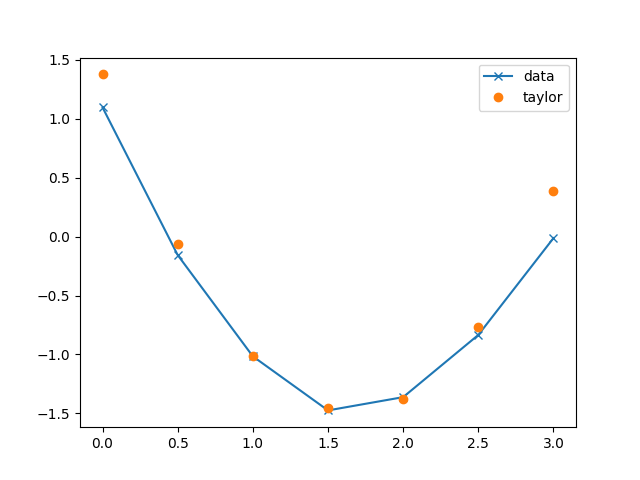
\includegraphics[width=\linewidth]{figures/taylor_expansion.png}
	\caption{Serie de Taylor de tercer grado}
	\label{fig:taylor_3rd_deg}
\end{figure}

\newpage 

\paragraph{Error cuadrático de la serie de Taylor de tercer grado}

El error cuadrático es $0.25296971634620236$ y se puede ver en la gráfica de abajo: 


\begin{figure}[H]
	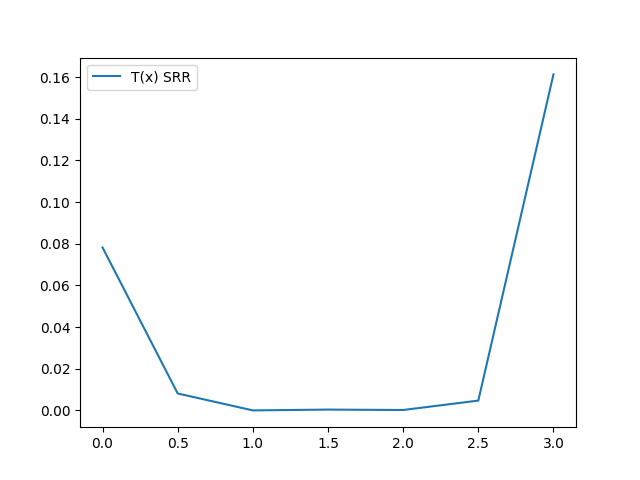
\includegraphics[width=\linewidth]{figures/taylor_quad_err.png}
	\caption{Error cuadrático de la serie de Taylor de tercer grado}
	\label{fig:taylor_3rd_deg_quad_err}
\end{figure}

\newpage 

\paragraph{Errores en respecto al ajuste por mínimos cuadrados}

Ahora procederemos a calcular y representar dos tipos de errores:

$$
S = \sum |y_k - f(x_k)|
$$

y 

$$
SRR = \sum (y_k - f(x_k))^2 
$$

donde la función $f(x_k)$ es la de ajuste por mínimos cuadrados usando los parámetros hallados en el apartado c). Haremos esto por cada aproximación.


\begin{figure}[H]
	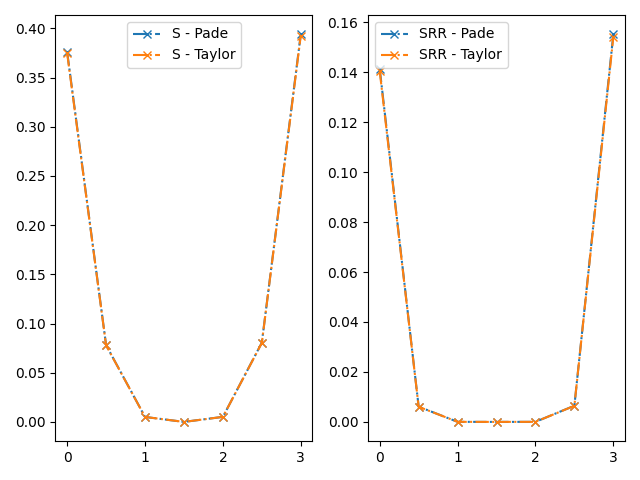
\includegraphics[width=\linewidth]{figures/approximation_errors.png}
	\caption{Errores en las aproximaciones}
	\label{fig:approximation_errors}
\end{figure}

Y los errores son:

\begin{itemize}
\item S - Pade: 0.938547
\item S - Taylor: 0.935348 
\item SRR - Pade: 0.309100 
\item SRR - Taylor: 0.306984 
\end{itemize}

\newpage 

\subsection{Discusión}

Lo primero de todo es que el error es mínimo cerca del punto de expansión $t_0 = 1.5$. Como hemos visto repetidamente en esta PEC, escoger bien el punto en torno al cual realizamos la aproximación es crucial. Segundo, la diferencia entre los errores es mínima, que muestra lo bueno que es el aproximante de Padé al ser de grado cuadrático en vez de cúbico como la aproximación de Taylor. Lo mas probable es que si tengamos que interpolar sobre un rango bastante amplio, se prefiera el aproximante de Padé al ser más estable mientras que el de Taylor es más fácil de calcular por ende mejor si el rango es un pequeño vecindario en torno al punto de expansión.